\section{SAT-based method}
\label{sec:submission-method}
\subsection{Order encoding and correctness (RQ1)}
For each vertex, introduce $x_{v,i}\Leftrightarrow[f(v)\leq i]$ for
$0\leq i<s$, and use constants $x_{v,-1}=\bot$, $x_{v,s}=\top$.
The clauses
\begin{equation}
 \neg x_{v,i}\lor x_{v,i+1},\qquad 0\leq i<s-1,
\end{equation}
force monotonicity. Since $f(v)=a$ is equivalent to
$x_{v,a}\land\neg x_{v,a-1}$, a forbidden label pair $(a,b)$ is excluded by
\begin{equation}\label{eq:submission-forbidden}
 \neg x_{u,a}\lor x_{u,a-1}\lor\neg x_{v,b}\lor x_{v,b-1}.
\end{equation}
Generate this clause for $|a-b|<h$ on edges and $|a-b|<k$ on $D_2$,
with $0\leq a,b\leq s$, simplifying boundary constants.
For $L(2,1)$ the unsimplified clause count is
\[
 |V|\max(s-1,0)+|E|A(s)+|D_2|(s+1),\qquad
 A(s)=\begin{cases}1,&s=0,\\3s+1,&s\geq1.\end{cases}
\]
General-parameter counts are given in Table~\ref{tab:submission-symbolic}.


\begin{proposition}\label{prop:submission-encoding}
The resulting CNF is satisfiable exactly when an $L(h,k)$-labeling of
span at most $s$ exists.
\end{proposition}
\begin{proof}
A labeling in $[0,s]$ supplies monotone threshold values and violates no
forbidden-pair clause. Conversely, each monotone threshold sequence
determines one label: the first true index, or $s$ if all variables are
false. A decoded violation falsifies its clause in
\eqref{eq:submission-forbidden}, so every decoded labeling is valid.
Translation establishes the statement for span rather than maximum label.
For $s=0$, any positive separation requirement produces an empty clause;
with no constrained pairs, the all-zero labeling is feasible.
\end{proof}

Implementation tests compare both search strategies with an exhaustive
oracle on all nonisomorphic graphs with at most five vertices for $L(2,1)$.
The generalized tests cover all such graphs up to four vertices for
$(1,1),(2,1),(3,2),(1,3),(0,2),(2,0),(0,0)$, using Glucose and CaDiCaL.
Assignment-level checks exhaust the eight three-vertex graphs with
$s=0,\ldots,4$ for $L(2,1)$, with additional $h,k$ checks on small graphs.
Separate tests check simplification equivalence, constructor reflections,
and assignment-ILP constraints. These finite tests support implementation
validation; the proposition establishes general equivalence.



\subsection{Bounds and span search}
For a graph with an edge, use $L=h+(\Delta-1)\min(h,k)$,
which is $h+(\Delta-1)k$ in the present domain. In the closed
neighborhood of a maximum-degree vertex, sorted labels have $\Delta$
gaps of at least $k$, at least one of which is incident to the center
and has size at least $h$. This proves the lower bound. A greedy labeling
chooses the smallest legal nonnegative label at each vertex in a fixed
order; its validated span supplies $U$.

The linear strategy tests $s=U-1$; the hybrid strategy used in the
benchmarks tests $s=\lfloor(L+U)/2\rfloor$. Each trial uses a fresh CNF
and solver. SAT supplies a validated labeling and reduces $U$ to its
actual span; UNSAT raises $L$ to $s+1$. Learned clauses are not reused
across trials. Figure~\ref{fig:submission-pipeline} summarizes the procedure.

\begin{proposition}\label{prop:submission-search}
Given valid initial bounds, an equivalent decision encoding and
satisfiability-preserving symmetry constraints, the span search reports
\OPT{} only for an optimal incumbent.
\end{proposition}
\begin{proof}
The invariant is $L\leq\lambda_{h,k}(G)\leq U$, with a labeling supporting
$U$. SAT preserves the upper inequality. UNSAT at $s$ excludes every
span at most $s$, preserving the lower inequality after $L=s+1$.
Equality $L=U$ proves optimality, including when the initial bounds meet.
An interrupted trial makes neither update and cannot be treated as UNSAT.
\end{proof}

\begin{figure}[htbp]
\centering
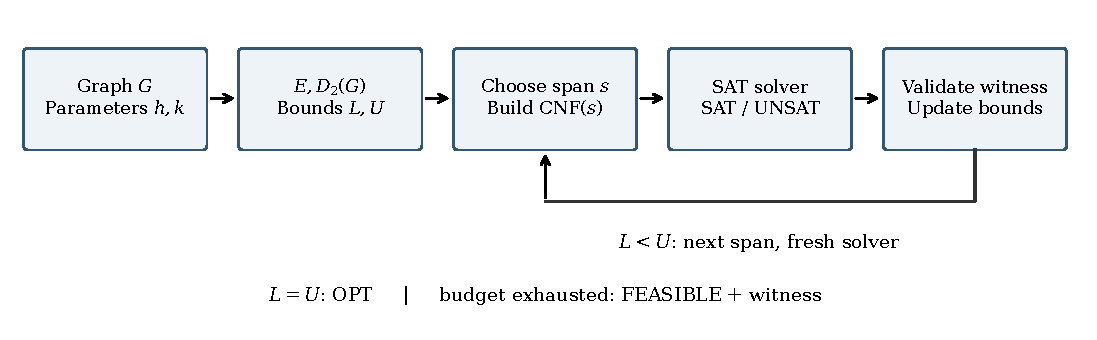
\includegraphics[width=\linewidth]{paper/generated/manuscript_figures/solver_pipeline.pdf}
\caption{Bounded SAT span search.}
\label{fig:submission-pipeline}
\tablenote{Only completed SAT or UNSAT decisions update the interval.
Timeout retains the last justified bounds and feasible labeling.}
\end{figure}

\subsection{Symmetry breaking}
\begin{proposition}\label{prop:submission-transitivity}
For a vertex-transitive graph, imposing $f(v_0)=0$ preserves the optimum
and feasibility of the decision problem with span at most $s$.
\end{proposition}
\begin{proof}
Translate a valid labeling so that some vertex $w$ has label zero.
An automorphism taking $v_0$ to $w$ preserves all distances; composing
the labeling with it assigns zero to $v_0$ without changing the span.
\end{proof}
Root fixing is used only for cycles in the symmetry experiment.
For $C_n$, choose $t$ attaining the minimum label and put
$g(i)=f((i+t)\bmod n)-f(t)$. Rotation and translation preserve feasibility
and span, so $g(0)=0$. Reflection about 0 then permits
$g(1)<g(n-1)$, since the two neighbors must have distinct labels.
Other tested families use only reflection orders: on $C_n\square H$,
$(i,j)\mapsto(-i\bmod n,j)$ exchanges $(1,0)$ and $(n-1,0)$;
on $C_n\circ H$, reflect the core and the attached copies together.
$H$ is a path or cycle. These automorphisms justify the selected order
without fixing a root. No additional constraint is used for
$P_n\square P_m$ or $P_n\circ H$.

Both configurations remove tautologies and duplicates and propagate
units to a fixed point. Fixed cycle-root thresholds are represented by
constants; retained unit clauses allow complete decoding. An order
constraint removes symmetric solutions, but may add clauses before
simplification. It does not guarantee halved CNF size or runtime.

\subsection{Combinatorial optimality certificates}
\begin{proposition}\label{prop:square-clique}
If $Q$ is a nonempty clique in the square $G^2$, then
$\lambda_{h,k}(G)\geq k(|Q|-1)$ for $h\geq k\geq1$.
A valid labeling attaining this bound is optimal.
\end{proposition}
\begin{proof}
Every pair in $Q$ is at distance one or two in $G$. Consecutive sorted
labels differ by at least $k$, and their $|Q|-1$ gaps sum to the bound.
A labeling attaining it supplies the matching upper bound.
\end{proof}
Any such clique suffices; it need not be proved maximum. The postprocessor
enumerates maximal cliques on the current small graphs and selects a
largest one, with lexicographic tie breaking. This potentially exponential
step is outside the timed solver comparison. A separate standard-library
checker verifies the original graph, clique membership and full labeling.
The following condition supplies additional witnesses.

\begin{proposition}[A sufficient color-order condition]
\label{prop:color-order}
Let $G$ be a nonempty simple undirected graph and $0<k\leq h\leq2k$.
Suppose $C_1,\ldots,C_r$ partition $V(G)$ into nonempty independent sets
of $G^2$. If $h>k$, suppose additionally that no edge of $G$ joins
consecutive classes $C_i,C_{i+1}$. Then
\[
 f(v)=k(i-1)\quad\text{for }v\in C_i
\]
is an $L(h,k)$-labeling of span $k(r-1)$.
If $G^2$ also contains a clique of size $r$, this span is optimal.
\end{proposition}
\begin{proof}
Vertices in the same class have distance greater than two, so equal
labels violate no constraint. Distinct classes have label difference at
least $k$, satisfying every distance-two constraint. If $h=k$, this also
suffices for edges. Otherwise, an edge cannot join consecutive classes
by assumption, and its endpoints differ by at least $2k\geq h$.
Every class is nonempty, so the span is $k(r-1)$. A square clique of size
$r$ gives the matching lower bound by Proposition~\ref{prop:square-clique}.
\end{proof}

\paragraph{Bounded construction.}
The implementation constructs a maximum-cardinality matching in the
complement of $G^2$. Each matched pair forms a class; unmatched vertices
form singleton classes. Every class is therefore independent in $G^2$.
This restricts the construction to classes of size at most two and need
not find a minimum coloring of $G^2$. Maximum matching only minimizes
the number of classes within this restricted partition scheme; its
optimality is unnecessary for checking a resulting labeling.

For $h>k$, define a compatibility graph on the classes, with an edge
between two classes exactly when no original graph edge joins them.
The required ordering is a Hamiltonian path in this compatibility graph.
A seeded insertion heuristic starts at a low-degree class, repeatedly
inserts an unplaced class into a compatible position, and restarts if
it cannot continue. It makes at most 100 attempts, with algorithmic seed 0
and canonical vertex and class ordering. The algorithmic seed is separate
from each archived graph-generation seed. A failure is reported as
\texttt{UNKNOWN}; it proves neither nonexistence of an ordering nor
infeasibility of the labeling instance. When $h=k$, no ordering search
is needed. Parameters outside the sufficient condition are not handled
by this construction; the general SAT/ILP formulations retain their
original domain.


The construction was developed after examining the unresolved instances.
Its subsequent whole-cohort application records both successes and
failures, but is not a held-out performance evaluation.


\subsection{Assignment ILP baseline}
Given a validated greedy upper bound $U$, let $y_{v,a}=1$ select label
$a\in\{0,\ldots,U\}$. The baseline minimizes $\ell_{\max}$ subject to
\begin{align}
 \sum_{a=0}^{U}y_{v,a}&=1 &&(v\in V),\\
 y_{u,a}+y_{v,b}&\leq1 &&(\{u,v\}\in E,\ |a-b|<h),\\
 y_{u,a}+y_{v,b}&\leq1 &&(\{u,v\}\in D_2,\ |a-b|<k),\\
 \sum_{a=0}^{U}a\,y_{v,a}&\leq\ell_{\max} &&(v\in V),\\
 y_{v,a}&\in\{0,1\},\qquad \ell_{\max}\in\{0,\ldots,U\}.
\end{align}
Exactly one label is chosen at each vertex, and all violating pairs are
forbidden. Every valid labeling in this domain supplies a feasible
assignment. Translation invariance therefore makes minimizing the maximum
label equivalent to minimizing span; no arbitrary vertex is fixed to zero.

To compare representation sizes, use a common domain $[0,s]$, set
$n=|V|$, and define
\[
 t_d=\min(s,d-1),\quad
 F(s,d)=(s+1)(2t_d+1)-t_d(t_d+1),\quad
 B=|E|F(s,h)+|D_2|F(s,k).
\]
Here $F(s,d)$ counts ordered label pairs with difference less than $d$.
Table~\ref{tab:submission-symbolic} gives the model sizes before
symmetry breaking or simplification.
\begin{table}[htbp]
\centering\small
\caption{Symbolic model sizes at span $s$.}
\label{tab:submission-symbolic}
\begin{tabular}{lll}
\toprule
Model & Variables & Clauses/rows\\\midrule
Order SAT & $ns$ & $n\max(s-1,0)+B$\\
Direct SAT (pairwise AMO) & $n(s+1)$ & $n(1+\binom{s+1}{2})+B$\\
Assignment ILP & $n(s+1)+1$ & $2n+B$\\
\bottomrule
\end{tabular}
\tablenote{Raw counts without symmetry breaking or preprocessing;
AMO means at most one. ILP includes one integer maximum-label variable;
variable bounds are not counted as rows.}
\end{table}
Direct SAT forbids a label pair with two literals, versus at most four
in order encoding. Other AMO encodings can alter the direct model size.
These are representation
counts, not equal-cost operations or a runtime ranking. Enumerating only
forbidden pairs costs $O((s+1)\min(s+1,2d-1))$ per constrained vertex
pair; this does not bound the complexity of solving the resulting model.


Under a one-based domain $1,\ldots,U'$, the optimal maximum label is
$\lambda_{h,k}+1$ for a nonempty graph. Our zero-based convention avoids
that offset. A Big-M formulation is also implemented: each separated
pair uses an orientation binary and two inequalities, with
$M=U+\max(h,k)$. It is not the baseline in the primary experiment;
no result here ranks all ILP formulations.
